\chapter{Previous Work}\label{ch:prevwork}

The previous work I've completed has focused primarily on efforts to run and
benchmark simple, once-through fuel cycle simulations with \Cyclus. Supporting
this effort has required not only additions to the \Cyclus code base to model
enrichment and reactor facilities, but also to the peripheral (i.e., linking
and input/output) and simulation-related infrastructure.

Significant, strategic improvements have been added to the \Cyclus code base
regarding interactions with dynamically-loadable libraries and reading XML-input
files. Basic simulation setup and execution has been revised to provide clear
phases of initialization. Tools have also been added to provide agent-based
management of building and instantiation of child agents, i.e., facilities in the
\Cyclus simulation. A (currently) separate library, named \Cyclopts, has been
developed to provide an interface to optimization solvers which currently
supports COIN-OR's linear and integer program solvers
\cite{lougee_common_2003}. Management of the actual building (instantiation) of
facilities within the simulation framework has been encapsulated in a
supplier/manager class pair. Finally, additional support has been added
specifically regarding to model enrichment-related calculations, allowing for
enrichment facilities to be developed in \Cycamore.

The combination of the above enhancements, in addition to developing an
enrichment and batch-based reactor facility models, as well as a managerial
institution model and demand-based region model, resulted in a \Cyclus
once-through fuel cycle simulation. In order to benchmark the basic simulation
infrastructure, the INPRO \cite{_international_2009} once-through benchmark was
used and compared with results from the VISION \cite{yacout_vision_2006}
code. Output closely matched for both reactor growth, gross material flows, and
SWUs utilized. Discrepancies were seen for the amount of natural uranium
utilized. The exercise of developing an input file for the the benchmark
specification was tedious due to the lack of published specifications. After a
review of other benchmarks, this was shown to be a common problem in addition to
a general lack fully specifying benchmark scenarios. Accordingly, a new
specification language was proposed and implemented, and a translation package
was implemented in order to translate that input into a \Cyclus input file.

\section{\Cyclus To Date}

\subsection{Dynamic Loading}\label{sec:prev-dynamic}

Libraries can be accessed in a static manner, i.e., they are connected to an
application during the linkage phase, or can be accessed in a dynamic manner,
i.e., they are connected at run time. Dynamic linkage, or dynamic loading, is a
well-known technique for to support connectable, modular components, or
plug-ins. \Cyclus utilizes a plug-in approach for its facility, institution, and
region agents. This design decision furthers the \Cyclus development goal of
providing an agnostic framework into which sophisticated users can develop
different models of agents to investigate a certain simulation-modeling change.

Work was performed in order to use class-based representation of dynamic
libraries, allowing for easy opening, closing, and access thereof. Each dynamic
library represents an agent type in \Cyclus, providing a constructor and
destructor. The DynamicModule class then provides the \Cyclus Core access to
these constructors and destructors to perform the appropriate operations at run
time. Because dynamic loading is treated differently on POSIX-based systems than
it is on Windows-based systems, specialty functions for library access were
provided for each system. The correct header file (UnixHelperFunctions.h or
WindowsHelperFunctions.h) is chosen during compilation. 

These changes simplified the client code that utilizes library access. The
\Cyclus Core application can now call appropriate library-related functions in
an agnostic manner. Specific, well-defined time points of module loading
(dynamic library opening) and unloading (dynamic library closing) were defined
in the \Cyclus application. These operations, called by the application,
currently reside in the Model class and could likely be refactored into a
specific handler class designed for this purpose.

\subsection{Input Reading}

A large overhaul to the input-reading code base was performed. \Cyclus currently
only supports XML input files that adhere to the RNG schema defined in \Cyclus
RNG file. However, it is a well-known best practice to provide an agnostic
application programming interface (API) that can be configured with specific
instances given some user-defined input. Accordingly, such an API was
constructed which currently supports XML input but can also support future input
types that are tree-based (e.g., JSON, CSV, etc.).

The top-level abstraction is encased in a QueryEngine class. Basic operations
are provided assuming a tree-based input formation, including querying the
number of child elements at the current reading level, the name of each element,
and access to each element. The application code is responsible for configuring
the appropriate input parser and populating an instance of a QueryEngine at its
root. The client code then populates input parameters through the QueryEngine
interface rather than an input-format specific interface.

Support for XML-file reading has been enhanced by separating various concerns
into appropriate classes. Four classes have been constructed with specific
purposes regarding input file reading: file loading (XMLFileLoader), file
validation (RelaxNGValidator), file parsing (XMLParser), and querying
(XMLQueryEngine). The application interfaces with the file loader, initializing
it with a given input file path and then invoking the loading of various
\Cyclus-specific parameters (e.g., simulation control parameters, material
recipes, agent modules, etc.). The loader is responsible for managing its parser
and providing client code with correctly-configured instances of
XMLQueryEngines. The parser is responsible for providing an interface to the
underlying C++ XML parsing library (currently libxml++ is used) and invoking the
appropriate validation routines on the parsed file. The validator is responsible
for providing access to the RNG-validation operations through, currently, libxml
and libxml++. Finally, the XML-specific derived QueryEngine class is responsible
for implementing XML-specific querying using the generic QueryEngine interface.

Other input file formats can be supported by providing the appropriate
format-specific derived QueryEngine class and adjusting the application code as
necessary. To developer could then choose how to implement the loading and
validation, if any, of the input file. The above structure is just one of many
ways to achieve such a goal.

\subsection{Enrichment Tools}\label{sec:prev-enrich}

The ability to calculate enrichment-related values is required to provide
important metrics for the simplest of fuel cycle simulations. Enrichment is the
process of artificially increasing the relative amount of Uranium-235 in a given
sample of Uranium. Naturally, Uranium contains approximately 0.72\% U-235, a
small amount (~0.005\%) U-234, and 99.274\% U-238. In light-water reactors
(LWRs), fissile U-235 is the primary fission fuel source, and thus reactors run
longer with higher amounts of U-235. Accordingly, reactor fuels are enriched to
~3-6\% U-235. It should be noted that enrichment of Uranium above 20\% is
restricted by international law due to its capacity to be used as a weapon in
high concentrations. In practice, however, Uranium-based nuclear weapons
generally have enrichments of greater than 90\%.

The enrichment process has one input, or feed, stream (usually natural Uranium)
and two output streams, the product and the excess Uranium, called tails. The
U-235 abundance, or assay of each of these streams as well as the mass of each stream
determines how much work is required to perform the enrichment, where
enrichment-work is calculated using Separative Work Units (SWUs). The feed,
product, and tails stream mass and assay values are related. Equation
\ref{eqs:enr-feed} shows the relation between product and feed masses, and
Equation \ref{eqs:enr-tails} shows the relation between product and tails
masses. 

\begin{equation}\label{eqs:enr-feed}
  F = P \frac{x_{p} - x_{t}}{x_{f} - x_{t}}
\end{equation}

\begin{equation}\label{eqs:enr-tails}
  T = P \frac{x_{p} - x_{f}}{x_{f} - x_{t}}
\end{equation}

Note that both equations depend on the U-235 assay ($x_i$s) of each
stream. Furthermore, given the assay of each stream, one needs to either set
the product or feed value (in the case of Equation \ref{eqs:enr-feed}) and the
product or tails value (in the case of Equation \ref{eqs:enr-tails}). In
practice, the feed and tail assays are set and an order for some quantity of
enriched product is requested. The resulting required feed and tail masses are
then calculated.

Enrichment plants measure their production in SWUs due to the quality
(enrichment level) variation of their product from order to order. The amount of
SWUs required to enrich a quantity of Uranium to a certain assay is a
function of all of the aforementioned variables (assays and masses of the
feed, product, and tails streams). The SWU calculation is shown in Equation
\ref{eqs:enr-swu}, where $V(x)$ is the Value Funtion defined in Equation
\ref{eqs:enr-value}.

\begin{equation}\label{eqs:enr-swu}
  SWU = P \; V(x_{p}) + T \; V(x_{t}) - F \; V(x_{f})
\end{equation}

\begin{equation}\label{eqs:enr-value}
  V(x) = (1 - 2x) \ln \left( \frac{1-x}{x} \right)
\end{equation}

Combining Equations \ref{eqs:enr-feed}, \ref{eqs:enr-tails}, and
\ref{eqs:enr-swu}, one can represent the SWU calculation as a function only of
the product mass and feed, product, and feed stream assays as shown in
Equation \ref{eqs:enr-swu-p}.

\begin{equation}\label{eqs:enr-swu-p}
  SWU = P \left( V(x_{p}) + \frac{x_{p} - x_{f}}{x_{f} - x_{t}} V(x_{t}) 
        - \frac{x_{p} - x_{t}}{x_{f} - x_{t}} V(x_{f}) \right)
\end{equation}

An Enrichment class was added to the \Cyclus set of utility toolkits under the
enrichment namespace. A simple Assay container class was also added, and is used
as the argument to many of the above calculations. The Enrichment toolkit allows
for the calculation of each of the abovementioned values and is used primarily
in the EnrichmentFacility that was added to \Cycamore to run the once-through
fuel cycle benchmarks.

\subsection{Facility Building and Supply/Demand Tools}

In order to support simple, once-through fuel cycle simulations, a nominal
capacity supply-demand interaction capability was needed. The use case of such a
system is to define demand for a given installed capacity, say in gigawatts of
produced power. Agents in a \Cyclus simulation generally have a natural
lifecycle, leaving the simulation at the end of their lifetimes. The system must
be able to respond to changes in installed capacities if it is to continue to
meet the simulated demand curves.

\subsubsection{Facilities as Prototypes}
should be there at home...

\subsubsection{Symbolic Functions}

The ability to represent symbolic functions was added to the \Cyclus Utiliy
toolkit. Functions are represented by a base Function class providing an
appropriate API. Linear, exponential, and piecewise function classes are
supported, where piecewise functions can utilize both linear and exponential
piecewise functions. Factory classes are provided to take a string of parameters
as read from an input file and return the appropriate symbolic function. A
simple example of the piecewise function support is provided in Figure
\ref{fig:piecewise}.

\begin{figure}[H]
  \begin{center}
    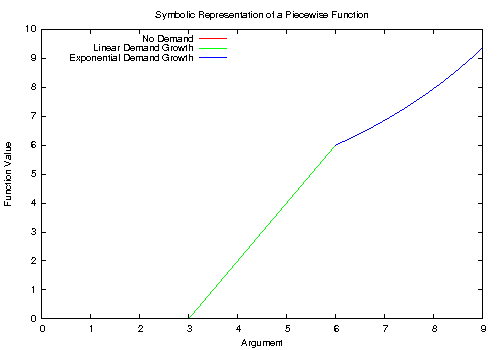
\includegraphics[width=\linewidth]{./chapters/prevwork/piecewise.png}
  \caption{An example of a piecewise function represented using the updated API.}
  \label{fig:piecewise}
  \end{center}
\end{figure}

\subsubsection{Tracking Commodity Production Capacity}

There is a need to track the current capacity of the production of a certain
commodity. Electrical power was offered the a prime example for this
once-through fuel cycle use case. Accordingly, a simple ``mixin'' class
\cite{ulrich_mixin-based_2001} called CommodityProducer was developed. It offers
an interface for accessing a list of commodities an entity produces and their
associated capacity to produce each commodity as well as the unit price of
commodity production. To date, the mixin has been used in conjunction with the
BatchReactor class, which serves as the reactor model for the once-through fuel
cycle simulations. The BatchReactor subclasses from both the base Facility class
as well as the CommodityProducer class.

A CommodityProducerManager class was also developed to manage a collection of
commodity producers. Its interface include registration and unregistration
methods to keep track of the producers it manages as well as a simple interface
for querying the current total capacity level of the commodity producers it
manages. It is also designed as a ``mixin'' class which has been utilized by the
ManagerInst class in \Cycamore, allowing the institution to keep track of the
capacity of facilities that produce certain commodities (e.g., electrical
power). This manager class is a use of the classic Observer design pattern
\cite{vlissides_design_1995}.

\subsubsection{Supply/Demand Tracking and Intelligent Build Decisions}

Three concerns remain in order to implement an appropriate model of responses to
changing supply capacity and demand for capacity. First, the current supply and
demand levels must be queryable. Second, if demand is greater than supply, some
new simulation entity must be built or introduced into the simulation. Third, a
decision must be made as to which entities should be built to meet a demand gap
if it exists.

A SupplyDemandManager class has been introduced to provide an interface for
querying the current supply capacity and demand for a given commodity. The class
is an Observer of CommodityProducerManagers, querying them when appropriate to
determine the full production capacity for the union of CommodityProducers
managed by the set of CommodityProducerManagers. Demand functions are also
registered for each commodity. An instance of a SupplyDemandManager is a private
member of the GrowthRegion class in \Cycamore, which supports building
facilities based on user-defined growth curves.

A Builder class has been introduced an interface for an entity that can build,
or instantiate into the simulation, instances of CommodityProducers. It is
designed as a ``mixin'' class and is utilized by the ManagerInst class in
\Cycamore. To date, institutions have been thought of as managers of facilities
by the \Cyclus development team, thus it is possible that the notion of facility
deployment management encapsulated in the current version of the ManagerInst
could be refactored into the Institution base class in the \Cyclus core
database. Such a decision will be informed by present and future use cases.

Finally, the BuilderManager class has been introduced to encapsulate the
decision making operations regarding building new facilities. It is an Observer
of Builder class instances, and an instance of the BuilderManager is used as a
private member by the GrowthRegion class in \Cycamore. The BuilderManager
interacts with the region's SupplyDemandManager to query the existence of unmet
demand. If it exists, it solves an integer program formulated as Equation
\ref{eqs:build-decision},

%%% 
\begin{subequations}\label{eqs:build-decision}
  \begin{align}
    %%
    \min \:\: & 
    \sum_{f \in F} n_f c_f
    & \\
    %%
    \text{s.t.} \:\: &
    \sum_{f \in F} n_f \phi_f \ge \Phi
    & \\
    %%
    &
    n_f > 0 \: \text{and} \: integer
    &
    \forall f \in F
    %%
  \end{align}
\end{subequations}
%%% 
  
where $\Phi$ is the unmet demand, $F$ is the set of facilities capable of
meeting the demand, and, for each facility in $F$, $c_f$ is the cost of
building, and $\phi_f$ is the nameplate capacity.  Finally, $n_f$ is the
optimized number of facilities to build of type $f$. The set of facilities and
their associated costs and capacities are queried through the managed Builder
instances.


\subsection{\Cyclopts}

\section{Benchmarking Efforts}\label{sec:prev-benchmark}

\subsection{VISION Once-Through}

\subsection{Benchmark Specification Language}
